% src/slides/source/final/core/01b_collaboration_strategies.tex

\begin{frame}{Collaboration Strategies}
  \SlideBody{\begin{VisualCanvas}
    \node[final heading] at (3.4,5.45) {Early Fusion};
    \node[final heading] at (7.4,5.45) {Intermediate Fusion};
    \node[final heading] at (11.4,5.45) {Late Fusion};
    \draw[draw=MoverCyan,line width=1.5pt] (5.8,5.10) -- (9.0,5.10);
    \node[inner sep=0pt] at (7.4,3.10)
      {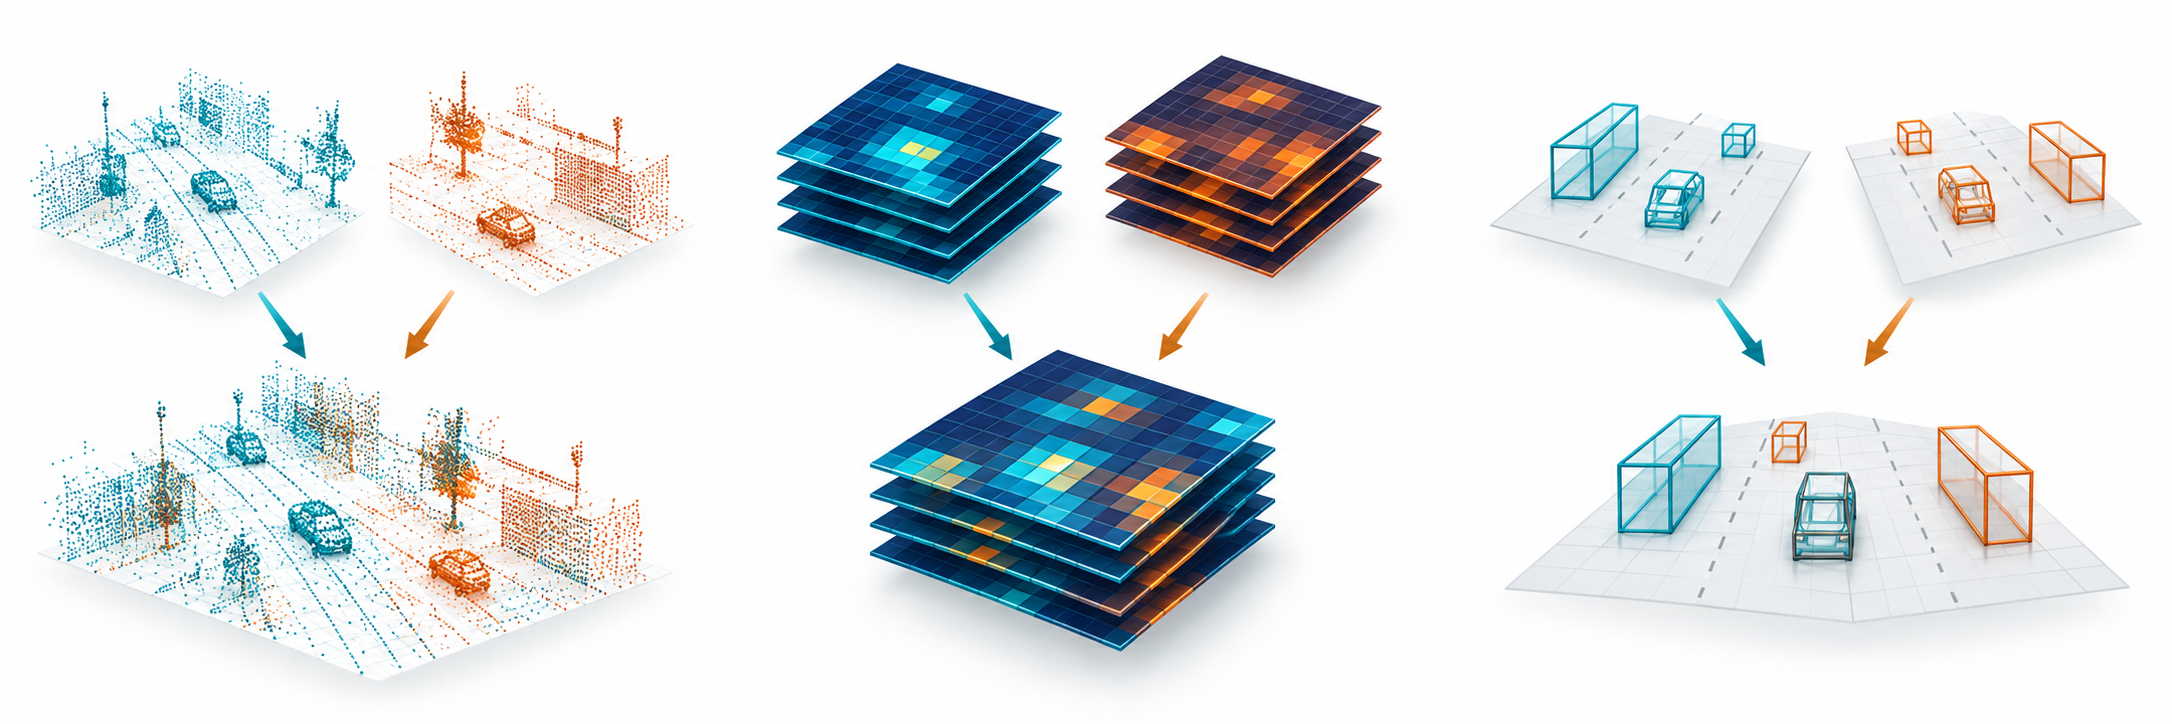
\includegraphics[width=12.0cm]{assets/illustrations/fusion-strategies.png}};
    \node[final caption] at (3.4,0.95) {Raw Points};
    \node[final caption] at (7.4,0.95) {Learned Features};
    \node[final caption] at (11.4,0.95) {Boxes + Scores};
    \node[visual small,anchor=center] at (3.4,0.52) {Before Encoding};
    \node[visual small,anchor=center] at (7.4,0.52) {Before Detection};
    \node[visual small,anchor=center] at (11.4,0.52) {After Detection};
  \end{VisualCanvas}}
  \SlideSource{Source: AI generated illustrations.}
\end{frame}
